\documentclass[10pt,a4paper]{article}
\usepackage[utf8]{inputenc}
\usepackage{amsmath}
\usepackage{amsfonts}
\usepackage{amssymb}
\usepackage{listings}
\usepackage{graphicx}
\lstset{showstringspaces=false,
		breaklines=true,
		postbreak=\raisebox{0ex}[0ex][0ex]{\ensuremath{\hookrightarrow\space}}}
    	
\begin{document}
\title{Intelligent Systems Assignment 3}
\author{Wessel Becker (1982362) \& Sander ten Hoor (2318555)}
\maketitle

\section{Matlab Code}
The following code was created for edge detection and boundary detection.

\subsection{simpleDifferentiation.m}
\lstinputlisting[language=Matlab]{./edgedetection/simpleDifferentiation.m}

\subsection{robert.m}
\lstinputlisting[language=Matlab]{./edgedetection/robert.m}

\subsection{sobel.m}
\lstinputlisting[language=Matlab]{./edgedetection/sobel.m}

\subsection{prewitt.m}
\lstinputlisting[language=Matlab]{./edgedetection/prewitt.m}

%\subsection{cannyEdgedetection.m}
%\lstinputlisting[language=Matlab]{./edgedetection/cannyEdgedetection.m}

\subsection{boundaryExtraction.m}
\lstinputlisting[language=Matlab]{./edgedetection/boundaryExtraction.m}

\section{Work done}

\section{Edge Detection}
\subsection{Simple Differentiation}
\begin{figure}
  \centering
    \makebox[\textwidth]{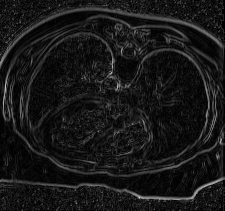
\includegraphics{./edgedetection/images/sd_no_noise}} \\
  \caption{Simple Differentiation, no noise}
  \label{fig:sd_no_noise}
\end{figure}

\begin{figure}
  \centering
    \makebox[\textwidth]{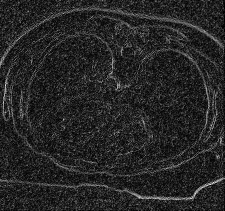
\includegraphics{./edgedetection/images/sd_001_noise}} \\
  \caption{Simple Differentiation, Gaussian noise with variance = 0.001}
  \label{fig:sd_001}
\end{figure}

\begin{figure}
  \centering
    \makebox[\textwidth]{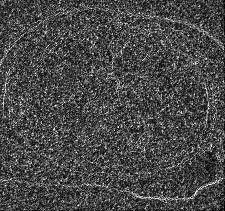
\includegraphics{./edgedetection/images/sd_005_noise}} \\
  \caption{Simple Differentiation, Gaussian noise with variance = 0.005}
  \label{fig:sd_005}
\end{figure}

\subsection{Roberts}
\begin{figure}
  \centering
    \makebox[\textwidth]{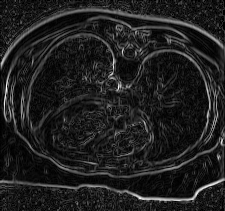
\includegraphics{./edgedetection/images/robert_no_noise}} \\
  \caption{Roberts, no noise}
  \label{fig:robert_no_noise}
\end{figure}

\begin{figure}
  \centering
    \makebox[\textwidth]{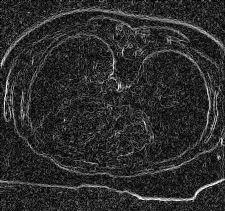
\includegraphics{./edgedetection/images/robert_001_noise}} \\
  \caption{Roberts, Gaussian noise with variance = 0.001}
  \label{fig:robert_001}
\end{figure}

\begin{figure}
  \centering
    \makebox[\textwidth]{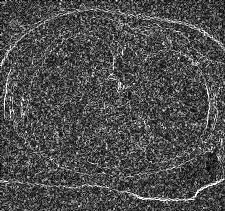
\includegraphics{./edgedetection/images/robert_005_noise}} \\
  \caption{Roberts, Gaussian noise with variance = 0.005}
  \label{fig:robert_005}
\end{figure}

\subsection{Sobel}
\begin{figure}
  \centering
    \makebox[\textwidth]{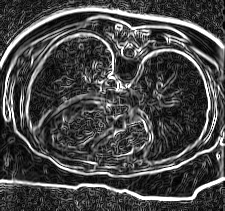
\includegraphics{./edgedetection/images/sobel_no_noise}} \\
  \caption{Sobel, no noise}
  \label{fig:sobel_no_noise}
\end{figure}

\begin{figure}
  \centering
    \makebox[\textwidth]{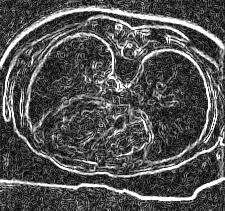
\includegraphics{./edgedetection/images/sobel_001_noise}} \\
  \caption{Sobel, Gaussian noise with variance = 0.001}
  \label{fig:sobel_001}
\end{figure}

\begin{figure}
  \centering
    \makebox[\textwidth]{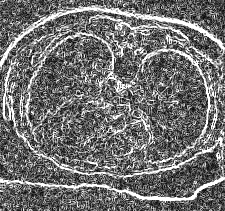
\includegraphics{./edgedetection/images/sobel_005_noise}} \\
  \caption{Sobel, Gaussian noise with variance = 0.005}
  \label{fig:sobel_005}
\end{figure}

\subsection{Prewitt}
\begin{figure}
  \centering
    \makebox[\textwidth]{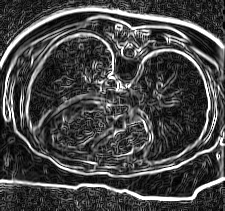
\includegraphics{./edgedetection/images/prewitt_no_noise}} \\
  \caption{Prewitt, no noise}
  \label{fig:prewitt_no_noise}
\end{figure}

\begin{figure}
  \centering
    \makebox[\textwidth]{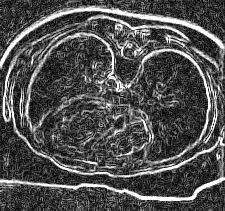
\includegraphics{./edgedetection/images/prewitt_001_noise}} \\
  \caption{Prewitt, Gaussian noise with variance = 0.001}
  \label{fig:prewitt_001}
\end{figure}

\begin{figure}
  \centering
    \makebox[\textwidth]{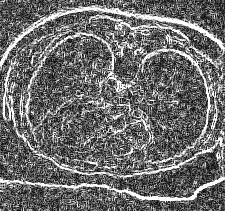
\includegraphics{./edgedetection/images/prewitt_005_noise}} \\
  \caption{Prewitt, Gaussian noise with variance = 0.005}
  \label{fig:prewitt_005}
\end{figure}
\end{document}